\documentclass{beamer}

\usepackage{minted}
\usepackage{amsmath}
\usepackage{amssymb}
\usepackage{graphicx}
\usepackage{tikz}
\usepackage{xcolor}
\usetheme{metropolis}

% \usetheme{Copenhagen}
% \usecolortheme{beaver}

\usetikzlibrary{shapes, arrows, positioning, decorations.pathreplacing,calligraphy}

\title{Linear Programming And The Simplex Algorithm}
\author{Ethan Lam \and Patrick Oweijane}
\institute{Christian Brothers University}
\date{April 27, 2022}

\begin{document}

\frame{\titlepage}

\begin{frame}
\frametitle{What Is Linear Programming?}
\begin{itemize}
    \item<1-> Linear programming is an optimization technique where we assign values to variables constrained by linear relationships.
    \item<2-> Linear programming problems often appear in applications such as operations research and finance.
    \item<2-> Problems will often come in the flavor of finding the best way to allocate resource under certain constraints.
\end{itemize}
\end{frame}

\begin{frame}{Example}
    \begin{itemize}
        \item<1-> Suppose you are managing 6000 acres of land belonging to a farm co-op.
        \item<2-> You can either plant corn or soybeans.
        \item<3-> You have the following resource budget: 
        \uncover<3->{
            \begin{tabular}{|c|c|c|c|}
                \hline
                & \textbf{Corn} & \textbf{Soybeans} & \textbf{Available} \\
                \hline
                Fertilizer/herbicide & 9 gal/acre & 3 gal/acre & 40500 gal \\
                Harvesting labor & $\frac{3}{4}$ hr/acre & 1 hr/acre & 5250 hr \\
                \hline
                Profit & 240 \$/acre & 160 \$/acre & \\ 
                \hline
            \end{tabular}
        }
        \item<4-> \textbf{How do you optimally plant corn and soybeans to maximize profit?}
    \end{itemize}
\end{frame}

\begin{frame}{Example (cont.)}
    We can write this optimization problem as
    \begin{equation*}
    \setlength\arraycolsep{1.5pt}
      \begin{array}{l@{\quad} r c r c r @{\quad\quad} r}
        \max          & 240x_1 & + &         160x_2 &      &    & \text{(Profit function)} \\
        \mathrm{s.t.} &   9x_1 & + &           3x_2 & \leq & 40500 & \text{(Fertilizer/herbicide constraint)}\\
                      &    \frac{3}{4}x_1 & + &           x_2 & \leq &  5250 & \text{(Labor constraint)}\\
                      & x_1 & + & x_2 & \leq & 6000 & \text{(Land constraint)}\\
                      &    x_1, x_2 &  & & \geq &  0 & \text{(Non-negativity constraint)}\\
      \end{array}
    \end{equation*}
    where your job is to find the best possible assignment of $x_1$ and $x_2$ which represent the amount of corn and soybeans you plant, respectively.
\end{frame}

\begin{frame}{Formalism}
    \begin{itemize}
        \item<1-> We will call instances of linear programming problems \textbf{linear programs}.
        \item<2-> Linear programs can be written in \textbf{standard form}.
        \begin{equation*}
            \setlength\arraycolsep{1.5pt}
            \begin{array}{l@{\quad} r c r} 
                \max          & c^{T}x & & \\
                \mathrm{s.t.} &  Ax & \leq & b \\
                              & x & \geq &  0 \\
            \end{array}
        \end{equation*}
        where $A$ is an $m \times n$ matrix, $x$ and $c$ are $n$ dimensional column vectors, and $b$ is an $m$ dimensional column vector.
        
        \begin{block}{Remark}<3->
            Let $b$ and $b'$ are $m$ dimensional vectors. By $b \leq b'$, we mean that for all $i = 1, 2, \ldots, m$
            \begin{align*}
                b_i \leq b'_i
            \end{align*}
        \end{block}
    \end{itemize}
\end{frame}

\begin{frame}{Formalism Made Concrete}
    \begin{columns}
        \column{0.45\textwidth} 
        Original linear program:
        \begin{equation*}
        \setlength\arraycolsep{1.5pt}
          \begin{array}{l@{\quad} r c r c r}
            \max          & 240x_1 & + &         160x_2 &      &    \\
            \mathrm{s.t.} &   9x_1 & + &           3x_2 & \leq & 40500 \\
                          &    \frac{3}{4}x_1 & + &           x_2 & \leq &  5250 \\
                          & x_1 & + & x_2 & \leq & 6000 \\
                          &    x_1, x_2 &  & & \geq &  0 \\
          \end{array}
        \end{equation*}
        
        \column{0.05\textwidth}
        \pause
        $\rightarrow$
        
        \column{0.50\textwidth} 
        \pause
        Standard form:
        \begin{equation*}
            \setlength\arraycolsep{1.5pt}
            \begin{array}{l@{\quad} r c r} 
                \max          & 
                \overbrace{\begin{bmatrix}
                    240 \\ 160
                \end{bmatrix}^{T}}^{c^T}
                \overbrace{\begin{bmatrix}
                    x_1 \\ x_2
                \end{bmatrix}}^{x} & & \\ \pause
                \mathrm{s.t.} &  
                \underbrace{\begin{bmatrix}
                    9 & 3 \\
                    \frac{3}{4} & 1 \\
                    1 & 1
                \end{bmatrix}}_{A}
                \begin{bmatrix}
                    x_1 \\ x_2
                \end{bmatrix} & \leq & 
                \underbrace{\begin{bmatrix}
                    40500 \\ 5250 \\ 6000
                \end{bmatrix}}_{b} \\ \pause
                              & 
                \begin{bmatrix}
                    x_1 \\ x_2
                \end{bmatrix} & \geq & 0 \\
            \end{array}
        \end{equation*}
    \end{columns}    
\end{frame}

\begin{frame}{Formalism (cont.)}
    \begin{itemize}
        \item<1-> The function we are optimizing is called the \textbf{objective function}.
        \item<2-> An assignment to $x$ that satisfies all constraints is called a \textbf{feasible solution}.
        \item<3-> Linear programs (in standard form) may be:
        \begin{itemize}
            \item<3-> Feasible ... optimal solution has finite objective value
            \item<4-> Infeasible ... no solutions
            \item<5-> Unbounded ... the objective value can be made infinite
        \end{itemize}
        \uncover<3->{
            \textit{(Fundamental theorem of linear programming)}
        }
    \end{itemize}
\end{frame}

\begin{frame}{Is Standard Form Too Restrictive?}
    \begin{itemize}
        \item<1-> What if we want to \textit{minimize} the objective function?
        \item<2-> What if we want variables to be \textit{unbounded}?
        \item<3-> What if we want variables to \textit{lie in an interval}?
        \item<4-> What if we want constraints to use $\geq$ or $=$?
        \item<5-> \textbf{All of these situations can be reformulated into a standard form equivalent!}
    \end{itemize}
\end{frame}

\begin{frame}{Slack Form Intuition}
    \begin{example}
        Consider
        \begin{align*}
            x_1 + x_2 \leq 6000
        \end{align*}
        \pause
        then
        \begin{align*}
            0 \leq \underbrace{6000 - x_1 - x_2}_{s}
        \end{align*}
        \pause
        where $s$ is the ``slack'' we have in increasing $x_1 + x_2$ until the constraint is violated. 
    \end{example}
\end{frame}

\begin{frame}{Slack Form}
    From the standard form we can construct the slack form: 
    \begin{equation*}
    \setlength\arraycolsep{1.5pt}
      \begin{array}{l@{\quad} r c r} 
        \max          & c^{T}x & & \\
        \mathrm{s.t.} &  s & = & b - Ax \\
                      & x, s & \geq &  0 \\
      \end{array}
    \end{equation*}
    where $s$ holds the ``slack'' variables which are added. 
    \pause
    \begin{itemize}
        \item Slack form turns our inequality constraints into equality constraints! \pause
        \item Variables on the left of the $=$ are called \textbf{basic variables} \pause
        \item Variables on the right of the $=$ are called \textbf{nonbasic variables} \pause
        \item \textit{Note: Only nonbasic variables appear in the objective function} \pause
        \item \textit{Note: As you solve a linear program, the nonbasic and basic variables will change.} \pause
        \item \textit{Note: Slack form makes solving linear programs easier.}
    \end{itemize}
\end{frame}

\begin{frame}{Slack Form Example}
    Standard form:
    \begin{equation*}
    \setlength\arraycolsep{1.5pt}
      \begin{array}{l@{\quad} r c r c r}
        \max          & 240x_1 & + &         160x_2 &      &    \\
        \mathrm{s.t.} &   9x_1 & + &           3x_2 & \leq & 40500 \\
                      &    \frac{3}{4}x_1 & + &           x_2 & \leq &  5250 \\
                      & x_1 & + & x_2 & \leq & 6000 \\
                      &    x_1, x_2 &  & & \geq &  0 \\
      \end{array}
    \end{equation*}
    
    \pause
    
    Slack form:
    \begin{equation*}
    \setlength\arraycolsep{1.5pt}
      \begin{array}{l@{\quad} r c r c r c r}
        \max          & 240x_1 & + &         160x_2 &      &    \\
        \mathrm{s.t.} & s_1 & = & 40500 & - & 9x_1 & - & 3x_2 \\
        & s_2 & = & 5250 & - & \frac{3}{4}x_1 & - & x_2 \\
        & s_3 & = & 6000 & - & x_1 & - & x_2 \\
        & x_1, x_2, s_1, s_2, s_3 & \geq & 0 &&&&  \\
      \end{array}
    \end{equation*}
\end{frame}

\begin{frame}{Simplex Algorithm}
    \begin{itemize}
        \item<1-> Developed by George Dantzig
        \item<2-> Runs in \textit{exponential} time but there exists polynomial time algorithms that solve linear programs
        \item<3-> Runs reasonably fast in practical applications
        \item<4-> Based on a fundamental operation called \textbf{pivoting}
    \end{itemize}
    \begin{block}{Interesting Theoretical Remarks}<5->
        \begin{itemize}
            \item<5-> The ability to solve linear programs in polynomial time means we have algorithms to solve problems reduced to linear programs quickly!
            \item<6-> Restricting the variables to integers makes solving linear programs \alert{NP-Hard}! (\textit{3-CNF-SAT can be reduced to determining if an integer linear program is feasible})
        \end{itemize}
    \end{block}
\end{frame}

% Macros to visually guide simplex example and to bring up visual with beamer overlays
\newcommand{\point}{{\color{red}\longrightarrow}}
\newcommand{\eColor}{yellow}
\newcommand{\lColor}{pink}
\tikzset{onslide/.code args={<#1>#2}{%
  \only<#1>{\pgfkeysalso{#2}} 
}}
\newcommand{\highlight}[3]{\tikz[baseline]{\node[rounded corners, rectangle, anchor=base, onslide=#1{fill=#2}]{#3}}}

\begin{frame}{Simplex Example}
    \begin{equation*}
        \setlength\arraycolsep{1.5pt}
          \begin{array}{l@{\quad} r c r c r c r}
            \max          & 240\highlight{<4->}{\eColor}{$x_1$} & + &         160x_2 &      &    \\
            \mathrm{s.t.} 
            & \uncover<5>{\point} \highlight{<8->}{\lColor}{$s_1$} & = & 40500 & - & 9 \highlight{<8->}{\eColor}{$x_1$} & - & 3x_2 \\
            & \uncover<6>{\point} s_2 & = & 5250 & - & \frac{3}{4}x_1 & - & x_2 \\
            & \uncover<7>{\point} s_3 & = & 6000 & - & x_1 & - & x_2 \\
            & x_1, x_2, s_1, s_2, s_3 & \geq & 0 &&&&  \\
          \end{array}
    \end{equation*}
    \pause
    \begin{itemize}
        \item<2-> Basic Solution: $(x_1, x_2, s_1, s_2, s_3) = (0, 0, 40500, 5250, 6000)$
        \item<3-> Basic Solution Value: $0$
        \item<4-> Entering Variable: \highlight{<4->}{\eColor}{$x_1$}
        \item<5-> First Constraint: $x_1$ can be at most $40500/9 = 4500$
        \item<6-> Second Constraint: $x_1$ can be at most $5250/(3/4) = 7000$
        \item<7-> Third Constraint: $x_1$ can be at most $6000/1 = 6000$
        \item<8-> Leaving Variable: \highlight{<8->}{\lColor}{$s_1$}
    \end{itemize}
\end{frame}

\begin{frame}{Simplex Example (cont.)}
    Increasing $x_1$ as much as possible means $s_1 = 0$ (there is no more ``slack''), and we can turn $s_1$ nonbasic and $x_1$ basic:
    \begin{equation*}
    \setlength\arraycolsep{1.5pt}
      \begin{array}{l@{\quad} r c r c r c r}
        \max          & 240\highlight{<1->}{\eColor}{$x_1$} & + &         160x_2 &      &    \\
        \mathrm{s.t.} & \highlight{<1->}{\eColor}{$x_1$} & = & 4500 & - & \frac{1}{9} \highlight{<1->}{\lColor}{$s_1$} & - & \frac{1}{3}x_2 \\
        & s_2 & = & 5250 & - & \frac{3}{4}x_1 & - & x_2 \\
        & s_3 & = & 6000 & - & x_1 & - & x_2 \\
        & x_1, x_2, s_1, s_2, s_3 & \geq & 0 &&&&  \\
      \end{array}
    \end{equation*} 
    \pause
    We now substitute all occurrences of $x_1$ to get
    \begin{equation*}
        \setlength\arraycolsep{1.5pt}
          \begin{array}{l@{\quad} r c r c r c r}
            \max          & -\frac{80}{3}\highlight{<2->}{\lColor}{$s_1$} & + &         80x_2 &    +  & 1080000    \\
            \mathrm{s.t.} & \highlight{<2->}{\eColor}{$x_1$} & = & 4500 & - & \frac{1}{9} \highlight{<2->}{\lColor}{$s_1$} & - & \frac{1}{3}x_2 \\
            & s_2 & = & 1875 & + & \frac{1}{12}s_1 & - & \frac{3}{4} x_2 \\
            & s_3 & = & 1500 & + & \frac{1}{9}s_1 & - & \frac{2}{3}x_2 \\
            & x_1, x_2, s_1, s_2, s_3 & \geq & 0 &&&&  \\
          \end{array}
    \end{equation*}
    \pause
    We now repeat this process ...
\end{frame}


\begin{frame}{Simplex Example (cont.)}
    \begin{equation*}
        \setlength\arraycolsep{1.5pt}
          \begin{array}{l@{\quad} r c r c r c r}
            \max          & -\frac{80}{3}s_1 & + &         80\highlight{<4->}{\eColor}{$x_2$} &    +  & 1080000    \\
            \mathrm{s.t.} 
            & \uncover<5>{\point} x_1 & = & 4500 & - & \frac{1}{9} s_1 & - & \frac{1}{3}x_2 \\
            & \uncover<6>{\point} s_2 & = & 1875 & + & \frac{1}{12}s_1 & - & \frac{3}{4} x_2 \\
            & \uncover<7>{\point} \highlight{<8->}{\lColor}{$s_3$} & = & 1500 & + & \frac{1}{9}s_1 & - & \frac{2}{3}\highlight{<8->}{\eColor}{$x_2$} \\
            & x_1, x_2, s_1, s_2, s_3 & \geq & 0 &&&&  \\
          \end{array}
    \end{equation*}
    \pause
    \begin{itemize}
        \item<2-> Basic Solution: $(x_1, x_2, s_1, s_2, s_3) = (4500, 0, 0, 1875, 1500)$
        \item<3-> Basic Solution Value: $1080000$
        \item<4-> Entering Variable: \highlight{<4->}{\eColor}{$x_2$}
        \item<5-> First Constraint: $x_2$ can be at most $4500/(1/3) = 13500$
        \item<6-> Second Constraint: $x_2$ can be at most $1875/(3/4) = 2500$
        \item<7-> Third Constraint: $x_2$ can be at most $(1500)/(2/3) = 2250$
        \item<8-> Leaving Variable: \highlight{<4->}{\lColor}{$s_3$}
    \end{itemize}
    \uncover<9->{After pivoting we get ...}
\end{frame}

\begin{frame}{Simplex Example (cont.)}
    \begin{equation*}
    \setlength\arraycolsep{1.5pt}
      \begin{array}{l@{\quad} r c r c r c r}
        \max          & -\frac{40}{3}s_1 & - &         120 s_3 &    +  & 1260000    \\
        \mathrm{s.t.} 
        & x_1 & = & 3750 & - & \frac{1}{6} s_1 & + & \frac{1}{2}s_3 \\
        & s_2 & = & \frac{375}{2} & - & \frac{1}{24}s_1 & + & \frac{9}{8} s_3 \\
        & x_2 & = & 2250 & + & \frac{1}{6}s_1 & - & \frac{3}{2}s_3 \\
        & x_1, x_2, s_1, s_2, s_3 & \geq & 0 &&&&  \\
      \end{array}
    \end{equation*}
    \pause
    \begin{itemize}
        \item<2-> Basic Solution: $(x_1, x_2, s_1, s_2, s_3) = (3750, 2250, 0, 375/2, 0)$
        \item<3-> Basic Solution Value: $1260000$
        \item<4-> We stop now because we cannot increase the objective function anymore.
        \item<5-> It turns out that this is the optimal solution!
        \item<6-> We should plant $x_1=3750$ acres of corn and $x_2=2250$ acres of soybeans yielding a profit of \$1,260,000.
    \end{itemize}
\end{frame}

\begin{frame}{Simplex Algorithm Overview}
    \begin{enumerate}
        \item<1-> Transform the linear program into a slack form where the basic solution is feasible.
        \item<2-> Find a nonbasic variable $x_e$, called the entering variable, in the objective function with positive coefficient. \label{step-pivot}
        \item<3-> Find the basic variable $x_l$, called the leaving variable, associated with the most restrictive constraint on $x_e$.
        \item<4-> Transform the linear program into an equivalent one by executing a pivot
        \item<5-> Go back to Step \ref{step-pivot} and if an entering variable cannot be found, stop.
        \item<6-> The basic solution is optimal so return it.
    \end{enumerate}
\end{frame}

\begin{frame}{Simplex Algorithm Technical Issues}
    \begin{itemize}
        \item<1-> How do you transform a linear program into a slack form where the basic solution is feasible?
        \item<2-> What is the ``most restrictive constraint''?
        \item<3-> Can the simplex algorithm run forever?
    \end{itemize} 
\end{frame}

\begin{frame}[fragile]{Our Implementation Goals}
    \begin{itemize}
        \item<1-> Linear programming can be extremely technical
        \item<2-> Easy-to-use interface to build linear programs
        \item<3-> Abstract away technical details of doing tedious transformations
        \item<4-> Use type-system to force users to use interface correctly
        \item<5-> Create test cases to validate our implementation
    \end{itemize} 
\end{frame}

\begin{frame}[fragile]{Our Implementation Usage Example}
    Creating a linear program:
    
    \begin{minted}[fontsize=\footnotesize]{Java}
LinearProgram p = new LinearProgram();
Variable corn = p.registerNonnegativeVariable("corn");
Variable soybeans = p.registerNonnegativeVariable("soybeans");
    \end{minted}
\end{frame}

\begin{frame}[fragile]{Our Implementation Usage Example}
    Adding constraints:
    \begin{minted}[fontsize=\scriptsize]{Java}
p.addConstraint(new Constraint(
        new ArrayList<>(Arrays.asList(corn, soybeans)),
        new ArrayList<>(Arrays.asList(9.0, 3.0)),
        Relation.LEQ,
        40500
));
p.addConstraint(new Constraint(
        new ArrayList<>(Arrays.asList(corn, soybeans)),
        new ArrayList<>(Arrays.asList(3.0/4.0, 1.0)),
        Relation.LEQ,
        5250
));
p.addConstraint(new Constraint(
        new ArrayList<>(Arrays.asList(corn, soybeans)),
        new ArrayList<>(Arrays.asList(1.0, 1.0)),
        Relation.LEQ,
        6000
));
    \end{minted}
\end{frame}

\begin{frame}[fragile]{Our Implementation Usage Example}
    Adding objective function:
    
    \begin{minted}[fontsize=\footnotesize]{Java}
p.setObjective(new ObjectiveFunction(
        ObjectiveGoal.MAXIMIZE,
        new ArrayList<>(Arrays.asList(corn, soybeans)),
        new ArrayList<>(Arrays.asList(240.0, 160.0))
));
    \end{minted}
\end{frame}

\begin{frame}[fragile]{Our Implementation Usage Example}
    Getting the solution:
    
    \begin{minted}[fontsize=\footnotesize]{Java}
System.out.println("Optimal profit: " + p.getObjectiveValue());
System.out.println("Corn: " + p.evaluateVariable(corn));
System.out.println("Soybeans: " + p.evaluateVariable(soybeans));
    \end{minted}
\end{frame}

\begin{frame}{Our Implementation Pipeline}
    \begin{enumerate}
        \item<1-> Obtain linear program $\mathcal{L}$ made by the user through our simple interface
        \item<2-> Compile $\mathcal{L}$ into an equivalent linear program $\mathcal{L'}$ in standard form
        \item<3-> Solve $\mathcal{L'}$ using the simplex algorithm
        \item<4-> Convert the answer found for $\mathcal{L'}$ back into an answer in $\mathcal{L}$
    \end{enumerate}
\end{frame}

\begin{frame}{Validation Methodology}
    \begin{itemize}
        \item<1-> Used exercises from a textbook\footnote{Mathematical Applications for the Management, Life, and Social Sciences (12th edition) by Harshbarger and Reynolds} and checked with the answers in the back of the book
        \item<2-> Used problems from the section on solving systems of difference constraints in CLRS
        \item<3-> Recasted example maximum flow problems in CLRS into linear programs
        \item<4-> Created stress tester that randomly generates maximum flow problems and validated solution with Max-Flow Min-Cut Theorem
    \end{itemize}
\end{frame}

\begin{frame}{Maximum Flow Problem As A Linear Programming Problem}
    \begin{itemize}
        \item<1-> Each edge $(u, v)$ has positive capacity $c_{uv}$
        \item<2-> Each edge $(u,v)$ is assigned a flow $f_{uv}$: $0 \leq f_{uv} \leq c_{uv}$
        \item<2-> \textit{Assume $f_{uv} = 0$ if $(u, v) \notin E$}
        \item<3-> All non-source and non-sink vertices $v$ must conserve flow: $\sum_{u \in V}f_{uv} = \sum_{w \in V}f_{vw}$
        \item<4-> Maximize total flow out of the source $s$: $\sum_{v \in V} f_{sv} - f_{vs}$
        \item<5-> All constraints and the objective function are linear relationships on the variables which means finding a maximum flow is reduced to solving a linear program! 
    \end{itemize}
\end{frame}

\begin{frame}{Stress Testing Our Implementation}
    \begin{columns}
        \column{0.5\textwidth}
        \begin{itemize}
            \item<1-> Large linear programs may expose implementation issues
            \item<2-> How do we generate large linear programs and also validate the answer?
            \item<3-> Generate large randomized flow network parameterized by $n$ and $k$ (Figure \ref{fig:stress-test-architecture})
            \item<4-> Max-Flow Min-Cut Theorem says that validating a maximum flow amounts to finding the non-existence of an augmenting path!
        \end{itemize}
        \column{0.5\textwidth}
        \onslide<3->{
            \begin{figure}
                \centering
                \resizebox{\textwidth}{!}{
                    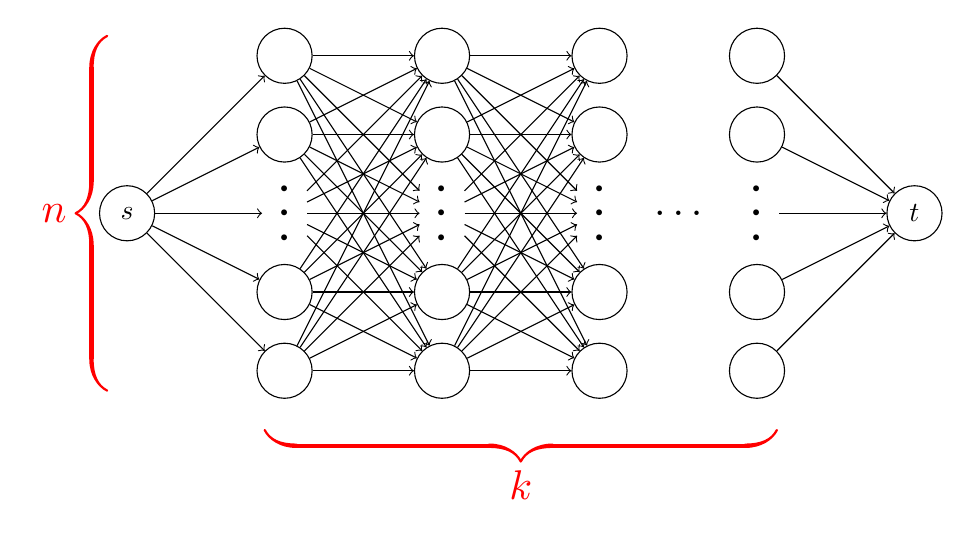
\begin{tikzpicture}
\node[draw, circle, minimum size=0.7cm] (s) at (0, 0) {$s$};
\node[draw, circle, minimum size=0.7cm] (t) at (10, 0) {$t$};

\node[draw, circle, minimum size=0.7cm] (l1v1) at (2, 2) {};
\node[draw, circle, minimum size=0.7cm] (l1v2) at (2, 1) {};
\node[draw, circle, minimum size=0.7cm] (l1v3) at (2, -1) {};
\node[draw, circle, minimum size=0.7cm] (l1v4) at (2, -2) {};
\path (l1v2) -- node[scale=2, rotate=90] (more1) {$\ldots$} (l1v3);

\node[draw, circle, minimum size=0.7cm] (l2v1) at (4, 2) {};
\node[draw, circle, minimum size=0.7cm] (l2v2) at (4, 1) {};
\node[draw, circle, minimum size=0.7cm] (l2v3) at (4, -1) {};
\node[draw, circle, minimum size=0.7cm] (l2v4) at (4, -2) {};
\path (l2v2) -- node[scale=2, rotate=90] (more2) {$\ldots$} (l2v3);

\node[draw, circle, minimum size=0.7cm] (l3v1) at (6, 2) {};
\node[draw, circle, minimum size=0.7cm] (l3v2) at (6, 1) {};
\node[draw, circle, minimum size=0.7cm] (l3v3) at (6, -1) {};
\node[draw, circle, minimum size=0.7cm] (l3v4) at (6, -2) {};
\path (l3v2) -- node[scale=2, rotate=90] (more3) {$\ldots$} (l3v3);


\node[draw, circle, minimum size=0.7cm] (l4v1) at (8, 2) {};
\node[draw, circle, minimum size=0.7cm] (l4v2) at (8, 1) {};
\node[draw, circle, minimum size=0.7cm] (l4v3) at (8, -1) {};
\node[draw, circle, minimum size=0.7cm] (l4v4) at (8, -2) {};
\path (l4v2) -- node[scale=2, rotate=90] (more4) {$\ldots$} (l4v3);

\path (more3) -- node[scale=1.5] {$\ldots$} (more4);

\foreach \v in {l1v1, l1v2, more1, l1v3, l1v4}
    \draw[->] (s) -- (\v);

\foreach \v in {l4v1, l4v2, more4, l4v3, l4v4}
    \draw[->] (\v) -- (t);

\foreach \u in {l1v1, l1v2, more1, l1v3, l1v4}
    \foreach \v in {l2v1, l2v2, more2, l2v3, l2v4}
        \draw[->] (\u) -- (\v);

\foreach \u in {l2v1, l2v2, more2, l2v3, l2v4}
    \foreach \v in {l3v1, l3v2, more3, l3v3, l3v4}
        \draw[->] (\u) -- (\v);


% Annotate parameters
\draw[decorate, decoration={calligraphic brace, mirror, raise=0.5cm, amplitude=0.4cm}, ultra thick, pen colour={red}] (l1v4.south west) -- (l4v4.south east) node[pos=0.5, below=0.8cm, red, scale=1.5]{$k$};

\draw[decorate, decoration={calligraphic brace, mirror, raise=2cm, amplitude=0.4cm}, ultra thick, pen colour={red}] (l1v1.north west) -- (l1v4.south west) node[pos=0.5, left=2.3cm, red, scale=1.5]{$n$};
\end{tikzpicture}
                }
                \caption{Stress test network architecture}
                \label{fig:stress-test-architecture}
            \end{figure}
        }
    \end{columns}
\end{frame}
\begin{frame}{Thanks!}
    \emph{Thanks for listening!}
    
    \begin{itemize}
        \item Implementation Code: \url{https://github.com/EthanTheMaster/LinearProgrammingSimplexAlgorithm}
    \end{itemize}
\end{frame}


\end{document}